\documentclass[a4paper]{article} 
\usepackage{amsmath,amsfonts,bm}
\usepackage{hyperref}
\usepackage{amsthm} 
\usepackage{geometry}
\usepackage{amssymb}
\usepackage{pstricks-add}
\usepackage{framed,mdframed}
\usepackage{graphicx,color} 
\usepackage{mathrsfs,xcolor} 
\usepackage[all]{xy}
\usepackage{fancybox} 
% \usepackage{CJKutf8}
\usepackage{xeCJK}
\newtheorem{theorem}{定理}
\newtheorem{lemma}{引理}
\newtheorem{corollary}{推论}
\newtheorem*{exercise}{习题}
\newtheorem{example}{例}
\geometry{left=2.5cm,right=2.5cm,top=2.5cm,bottom=2.5cm}
\setCJKmainfont[BoldFont=Adobe Heiti Std R]{Adobe Song Std L}
\renewcommand{\today}{\number\year 年 \number\month 月 \number\day 日}
\newcommand{\D}{\displaystyle}
\newcommand{\ds}{\displaystyle} \renewcommand{\ni}{\noindent}
\newcommand{\pa}{\partial} \newcommand{\Om}{\Omega}
\newcommand{\om}{\omega} \newcommand{\sik}{\sum_{i=1}^k}
\newcommand{\vov}{\Vert\omega\Vert} \newcommand{\Umy}{U_{\mu_i,y^i}}
\newcommand{\lamns}{\lambda_n^{^{\scriptstyle\sigma}}}
\newcommand{\chiomn}{\chi_{_{\Omega_n}}}
\newcommand{\ullim}{\underline{\lim}} \newcommand{\bsy}{\boldsymbol}
\newcommand{\mvb}{\mathversion{bold}} \newcommand{\la}{\lambda}
\newcommand{\La}{\Lambda} \newcommand{\va}{\varepsilon}
\newcommand{\be}{\beta} \newcommand{\al}{\alpha}
\newcommand{\dis}{\displaystyle} \newcommand{\R}{{\mathbb R}}
\newcommand{\N}{{\mathbb N}} \newcommand{\cF}{{\mathcal F}}
\newcommand{\gB}{{\mathfrak B}} \newcommand{\eps}{\epsilon}
\renewcommand\refname{参考文献}
\begin{document}
\title{\huge{\bf{用复数解一道平面几何题}}} \author{\small{叶卢
    庆\footnote{叶卢庆(1992---),男,杭州师范大学理学院数学与应用数学专业
      本科在读,E-mail:h5411167@gmail.com}}\\{\small{杭州师范大学理学院,浙
      江~杭州~310036}}}
\maketitle
如图,$ABC$ 是任意三角形,以$AC,AB$ 为边向外作正方形.$I,H$ 分别为正方形
中心.点$J$ 为 $BC$ 中点.求证$IJ$ 垂直于 $HJ$ 且 $|IJ=HJ|$.\\
\newrgbcolor{zzttqq}{0.6 0.2 0}
\psset{xunit=1.0cm,yunit=1.0cm,algebraic=true,dotstyle=o,dotsize=3pt 0,linewidth=0.8pt,arrowsize=3pt 2,arrowinset=0.25}
\begin{pspicture*}(2.13,-3.69)(19.02,3.83)
\pspolygon[linecolor=zzttqq,fillcolor=zzttqq,fillstyle=solid,opacity=0.1](9.81,0.06)(13.01,-2.17)(9.77,-2.8)
\pspolygon[linecolor=zzttqq,fillcolor=zzttqq,fillstyle=solid,opacity=0.1](9.81,0.06)(13.01,-2.17)(15.25,1.03)(12.04,3.27)
\pspolygon[linecolor=zzttqq,fillcolor=zzttqq,fillstyle=solid,opacity=0.1](9.77,-2.8)(9.81,0.06)(6.94,0.11)(6.9,-2.76)
\psline[linecolor=zzttqq](9.81,0.06)(13.01,-2.17)
\psline[linecolor=zzttqq](13.01,-2.17)(9.77,-2.8)
\psline[linecolor=zzttqq](9.77,-2.8)(9.81,0.06)
\psline[linecolor=zzttqq](9.81,0.06)(13.01,-2.17)
\psline[linecolor=zzttqq](13.01,-2.17)(15.25,1.03)
\psline[linecolor=zzttqq](15.25,1.03)(12.04,3.27)
\psline[linecolor=zzttqq](12.04,3.27)(9.81,0.06)
\psline[linecolor=zzttqq](9.77,-2.8)(9.81,0.06)
\psline[linecolor=zzttqq](9.81,0.06)(6.94,0.11)
\psline[linecolor=zzttqq](6.94,0.11)(6.9,-2.76)
\psline[linecolor=zzttqq](6.9,-2.76)(9.77,-2.8)
\psline(12.53,0.55)(11.39,-2.49)
\psline(11.39,-2.49)(8.35,-1.35)
\begin{scriptsize}
\psdots[dotstyle=*,linecolor=blue](9.81,0.06)
\rput[bl](9.86,0.14){\blue{$A$}}
\psdots[dotstyle=*,linecolor=blue](13.01,-2.17)
\rput[bl](13.06,-2.1){\blue{$B$}}
\psdots[dotstyle=*,linecolor=blue](9.77,-2.8)
\rput[bl](9.82,-2.73){\blue{$C$}}
\psdots[dotstyle=*,linecolor=darkgray](15.25,1.03)
\rput[bl](15.3,1.1){\darkgray{$D$}}
\psdots[dotstyle=*,linecolor=darkgray](12.04,3.27)
\rput[bl](12.1,3.34){\darkgray{$E$}}
\psdots[dotstyle=*,linecolor=darkgray](6.94,0.11)
\rput[bl](6.99,0.18){\darkgray{$F$}}
\psdots[dotstyle=*,linecolor=darkgray](6.9,-2.76)
\rput[bl](6.95,-2.69){\darkgray{$G$}}
\psdots[dotstyle=*,linecolor=darkgray](12.53,0.55)
\rput[bl](12.58,0.62){\darkgray{$H$}}
\psdots[dotstyle=*,linecolor=darkgray](8.35,-1.35)
\rput[bl](8.4,-1.27){\darkgray{$I$}}
\psdots[dotstyle=*,linecolor=darkgray](11.39,-2.49)
\rput[bl](11.44,-2.42){\darkgray{$J$}}
\end{scriptsize}
\end{pspicture*}
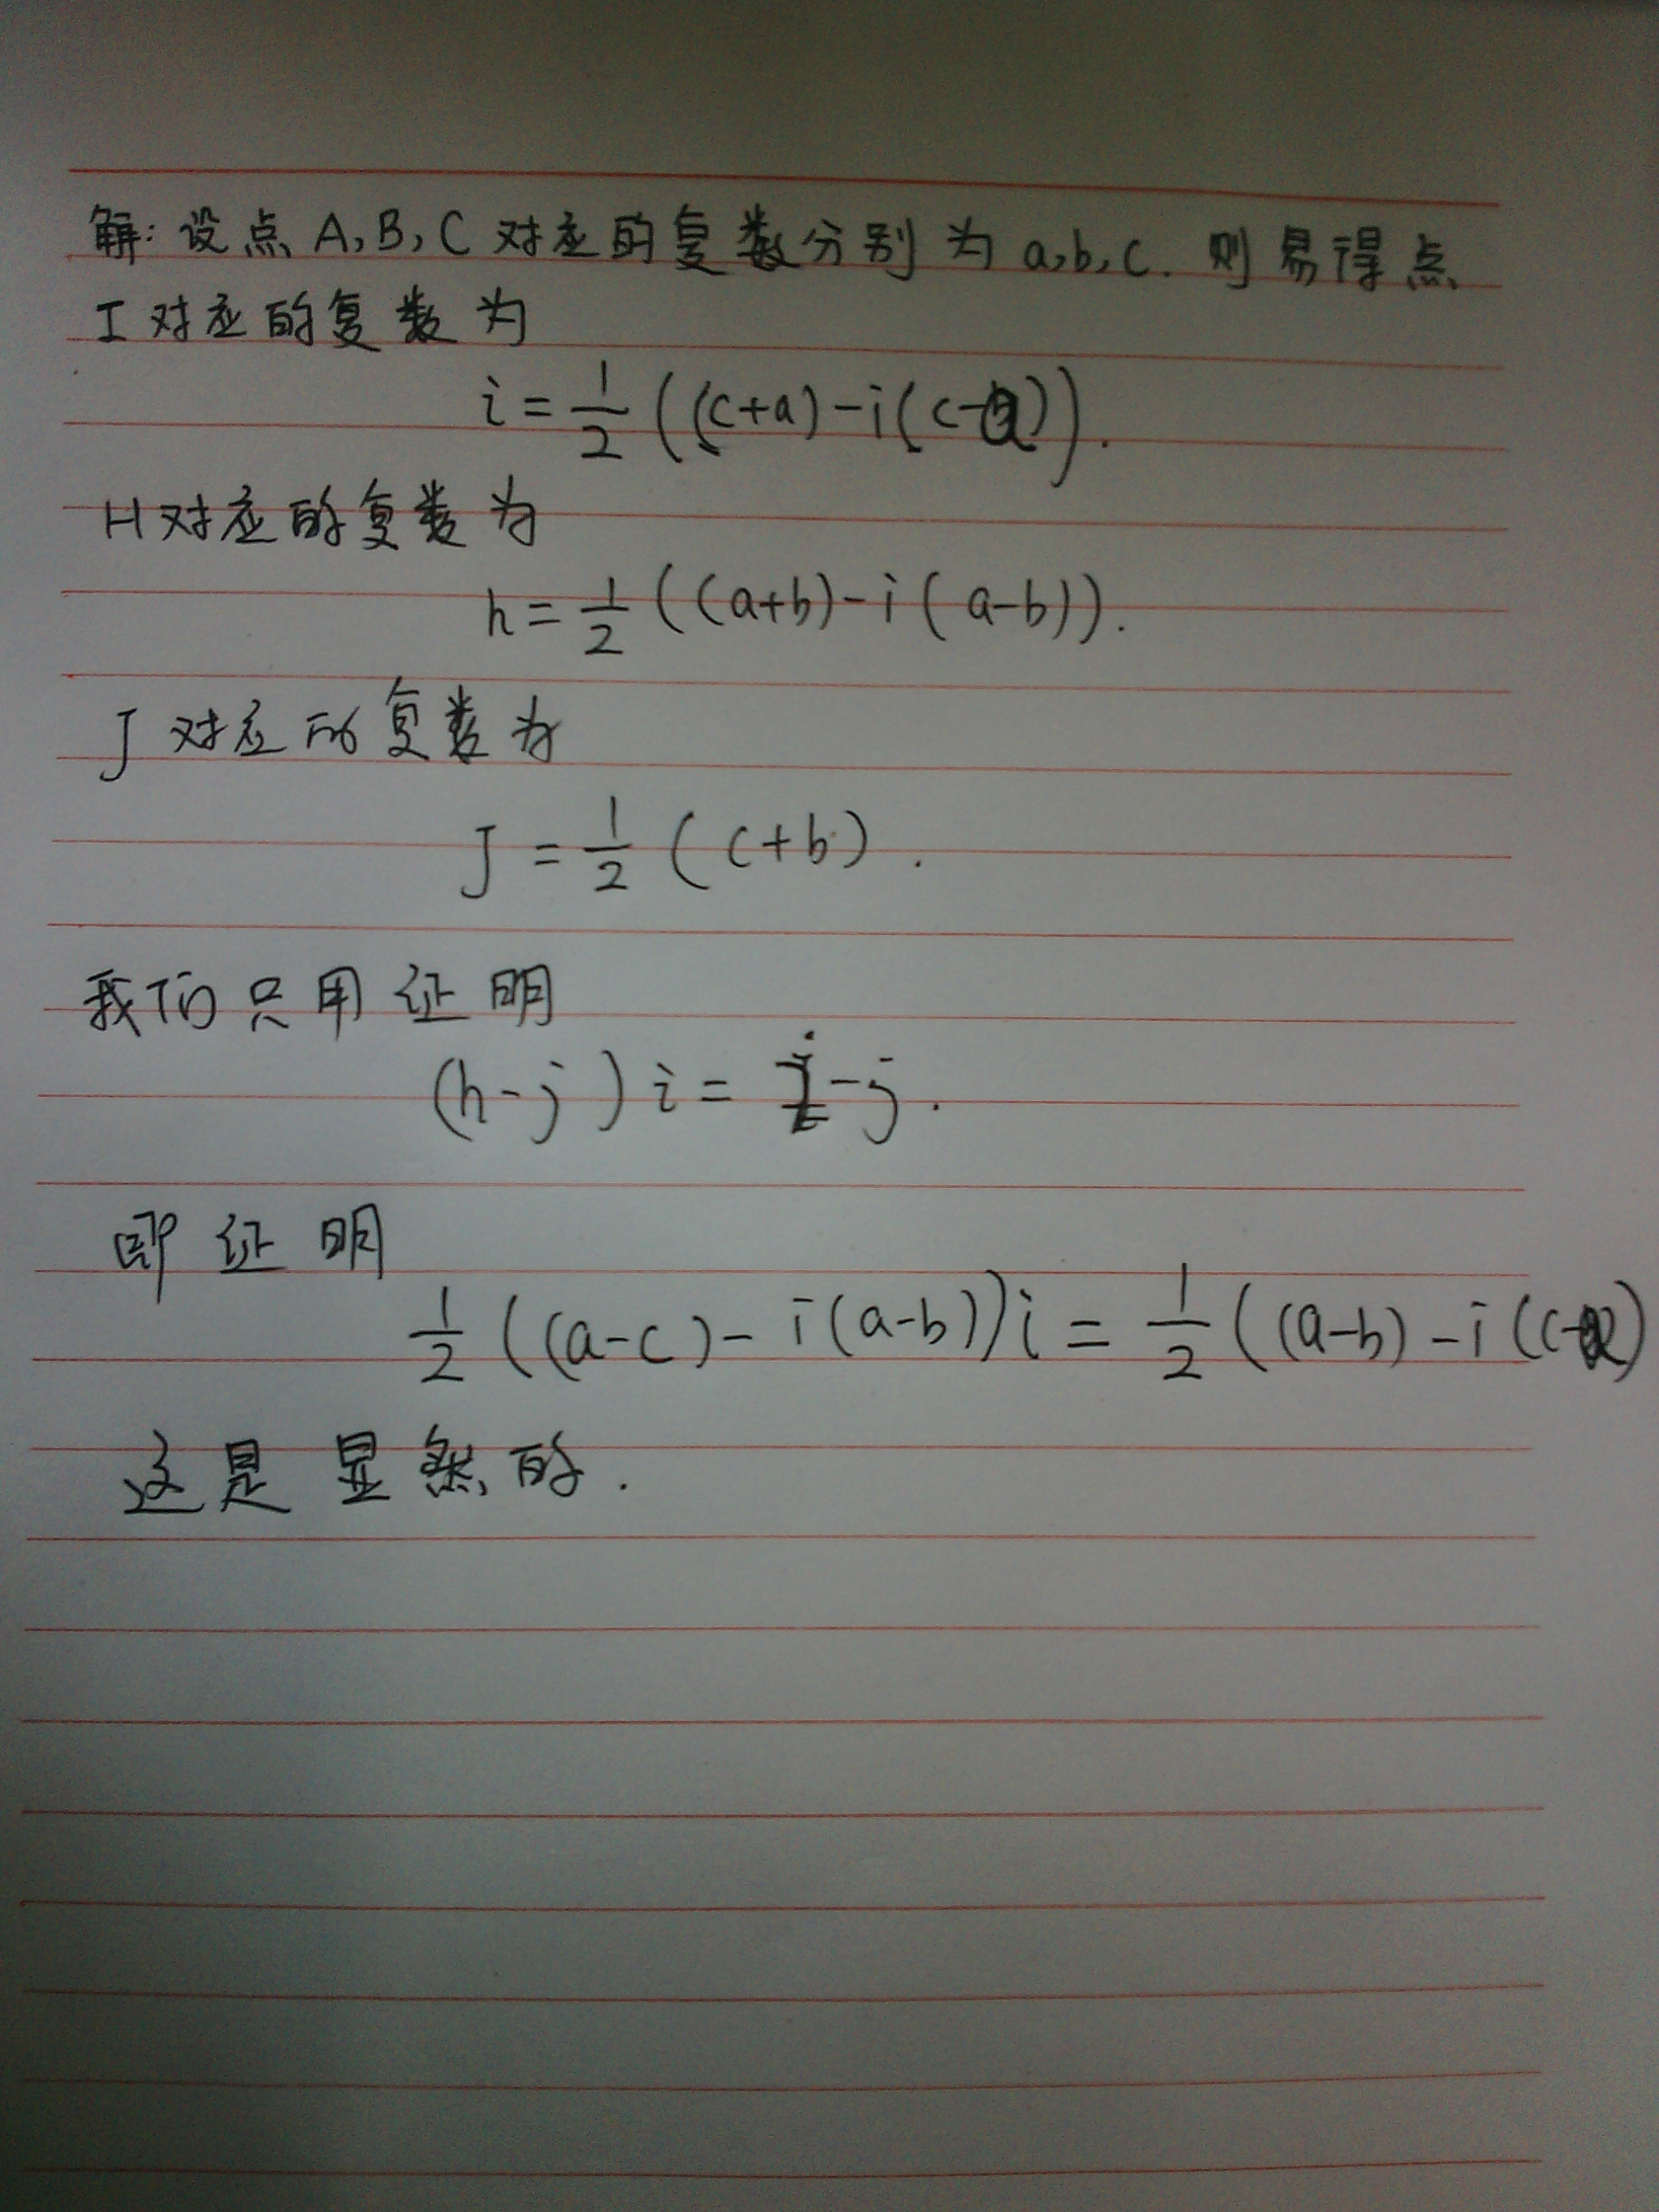
\includegraphics[width=1\textwidth]{/home/luqing/math/visual-complex-analysis/IMG20140224140132.jpg}
\end{document}








